\section{Results}
\label{sec:results}
The results of the verification method introduced in Sec.~\ref{sec:methods_verification}
are presented next.
\subsection{Straight Wire Segment}
First, the results of the verification of the straight wire segment methods are presented.
The normalized vertical component of the magnetic vector potential, $\tilde{A}_z$,
and the normalized tangential component magnetic field, $\tilde{B}_\varphi$, of a straight wire segment
have been evaluated using \eqn{sws_A_z_switchover} and \eqn{sws_B_phi_switchover}, respectively,
on all test points in $T_\mathrm{SWS}$ (see Sec.~\ref{sec:methods_verification}).
Fig.~(\ref{fig:StraightWireSegment_A_z_Java}) shows the deviation
according to the error metric~\eqn{error_metric}
between the reference data computed for $\tilde{A}_z$ using \eqn{sws_A_z_ref}
and the results from the \texttt{float64} implementation of \eqn{sws_A_z_switchover}.
\begin{figure}[htbp]
 \centering
 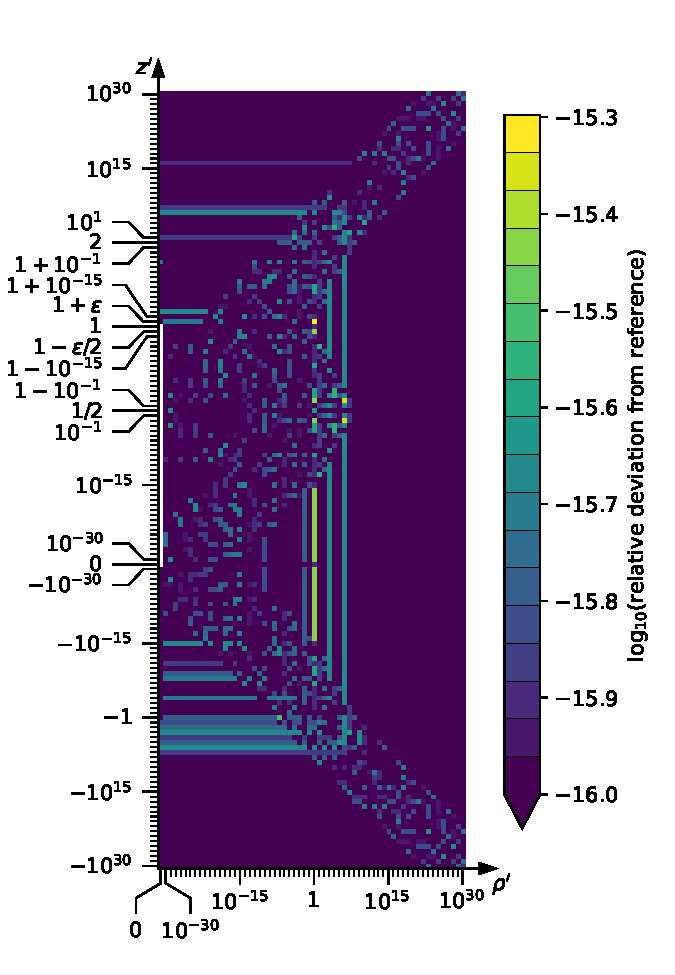
\includegraphics[height=0.8\textwidth]{img/StraightWireSegment_A_z_Java.pdf}
 \caption{Deviation between Java implementation of \eqn{sws_A_z_switchover} and \eqn{sws_A_z_ref}
          for the computation of $\tilde{A}_z$ of a straight wire segment
          in the error metric given by~\eqn{error_metric}.}
 \label{fig:StraightWireSegment_A_z_Java}
\end{figure}
It is observed that the relative error is less that $10^{-15}$ for all test points under consideration.
Fig.~(\ref{fig:StraightWireSegment_B_phi_Java}) shows the deviation
according to the error metric~\eqn{error_metric}
between the reference data computed for $\tilde{B}_\varphi$ using \eqn{sws_B_phi_ref}
and the results from the \texttt{float64} implementation of \eqn{sws_B_phi_switchover}.
\begin{figure}[htbp]
 \centering
 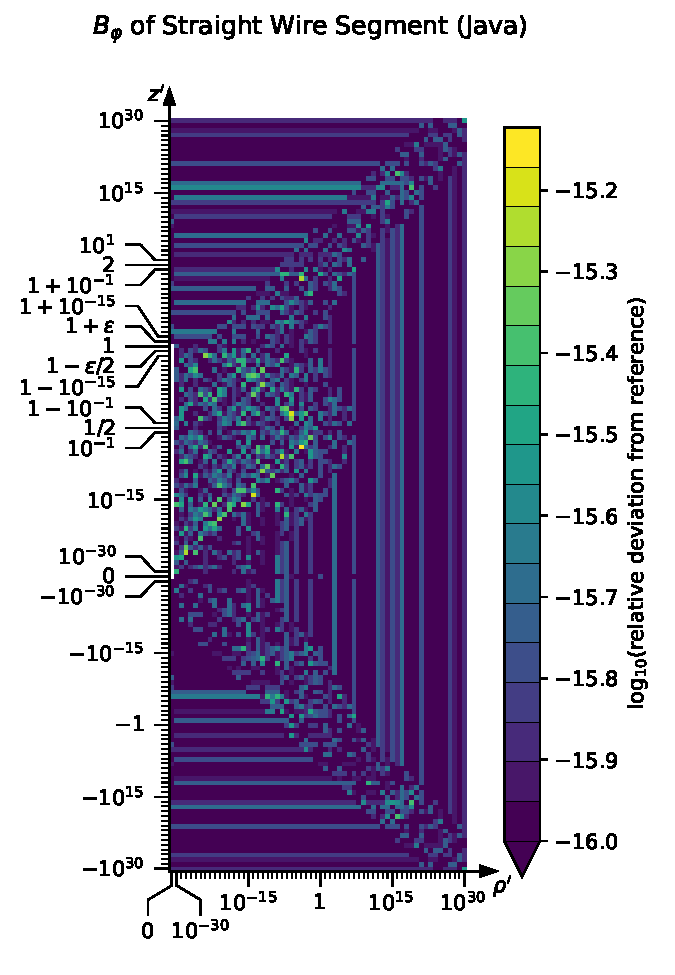
\includegraphics[height=0.8\textwidth]{img/StraightWireSegment_B_phi_Java.pdf}
 \caption{Deviation between Java implementation of \eqn{sws_B_phi_switchover} and \eqn{sws_B_phi_ref}
          for the computation of $\tilde{B}_\varphi$ of a straight wire segment
          in the error metric given by~\eqn{error_metric}.}
 \label{fig:StraightWireSegment_B_phi_Java}
\end{figure}
It is observed that the relative error is less that $10^{-15}$ for all test points under consideration.

\subsection{Circular Wire Loop}
Next, the results of the verification of the circular wire loop methods are presented.
The normalized tangential component of the magnetic vector potential, $\tilde{A}_\varphi$,
and the normalized radial and vertical components of the magnetic field, $\tilde{B}_\rho$ and $\tilde{B}_z$,
of a circular wire loop have been evaluated using \eqn{A_phi_final}, \eqn{cwl_B_rho_switchover}
and \eqn{cwl_B_z_switchover}, respectively,
on all test points in $T_\mathrm{CWL}$ (see Sec.~\ref{sec:methods_verification}).
Fig.~(\ref{fig:CircularWireLoop_A_phi_Java}) shows the deviation
according to the error metric~\eqn{error_metric}
between the reference data computed for $\tilde{A}_\varphi$ using \eqn{A_phi_ref}
and the results from the \texttt{float64} implementation of \eqn{A_phi_final}.
\begin{figure}[htbp]
 \centering
 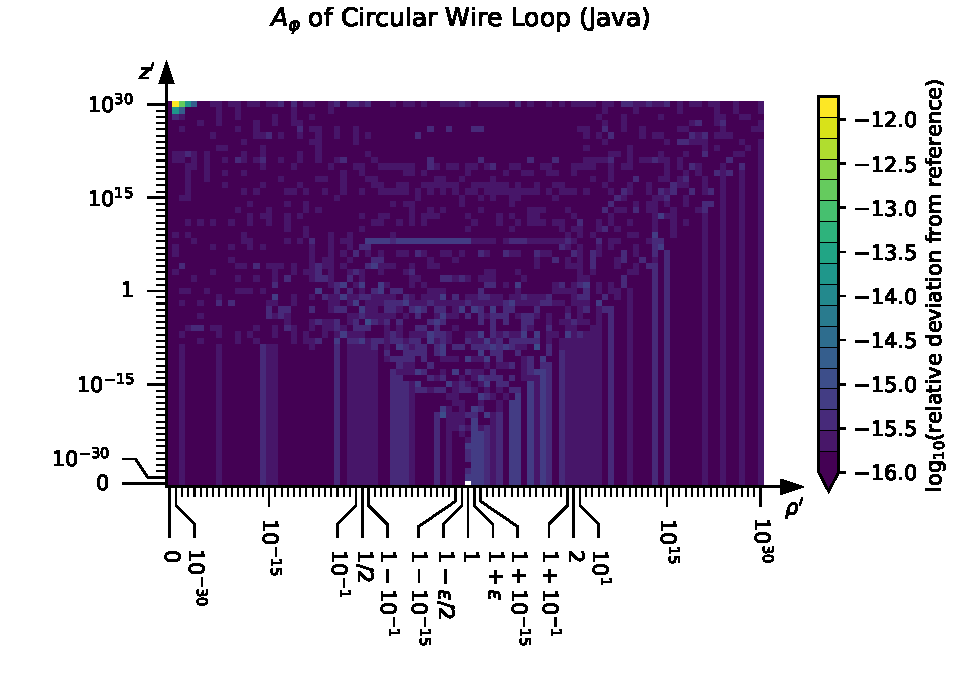
\includegraphics[width=0.8\textwidth]{img/CircularWireLoop_A_phi_Java.pdf}
 \caption{Deviation between Java implementation of \eqn{A_phi_final} and \eqn{A_phi_ref}
          for the computation of $\tilde{A}_\varphi$ of a circular wire loop
          in the error metric given by~\eqn{error_metric}.}
 \label{fig:CircularWireLoop_A_phi_Java}
\end{figure}
Fig.~(\ref{fig:CircularWireLoop_B_rho_Java}) shows the deviation
according to the error metric~\eqn{error_metric}
between the reference data computed for $\tilde{B}_\rho$ using \eqn{B_rho_ref}
and the results from the \texttt{float64} implementation of \eqn{cwl_B_rho_switchover}.
\begin{figure}[htbp]
 \centering
 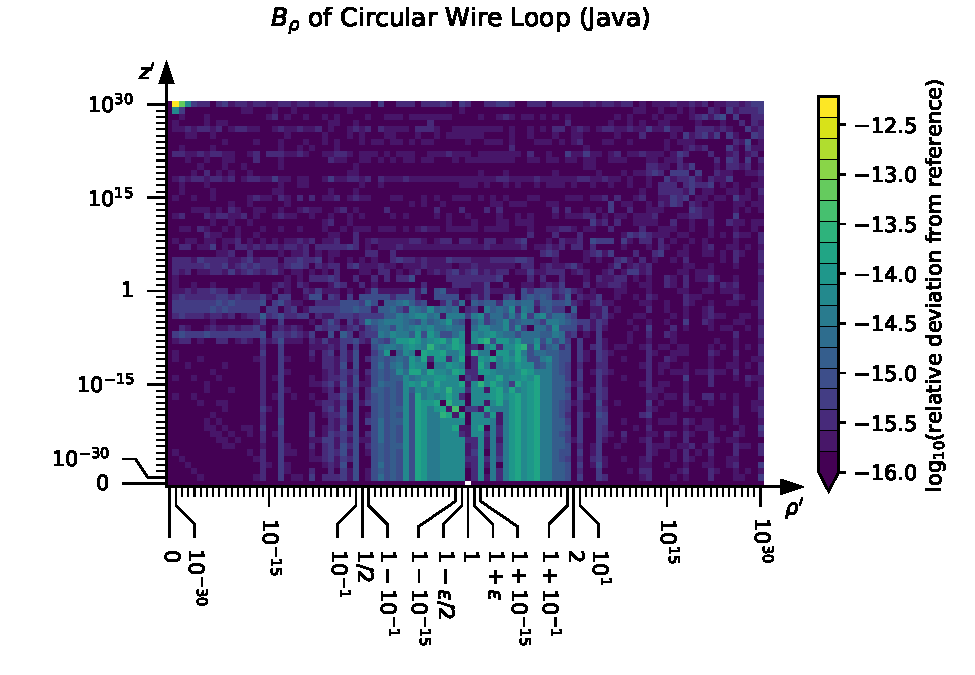
\includegraphics[width=0.8\textwidth]{img/CircularWireLoop_B_rho_Java.pdf}
 \caption{Deviation between Java implementation of \eqn{cwl_B_rho_switchover} and \eqn{B_rho_ref}
          for the computation of $\tilde{B}_\rho$ of a circular wire loop
          in the error metric given by~\eqn{error_metric}.}
 \label{fig:CircularWireLoop_B_rho_Java}
\end{figure}
Fig.~(\ref{fig:CircularWireLoop_B_z_Java}) shows the deviation
according to the error metric~\eqn{error_metric}
between the reference data computed for $\tilde{B}_z$ using \eqn{B_z_ref}
and the results from the \texttt{float64} implementation of \eqn{cwl_B_z_switchover}.
\begin{figure}[htbp]
 \centering
 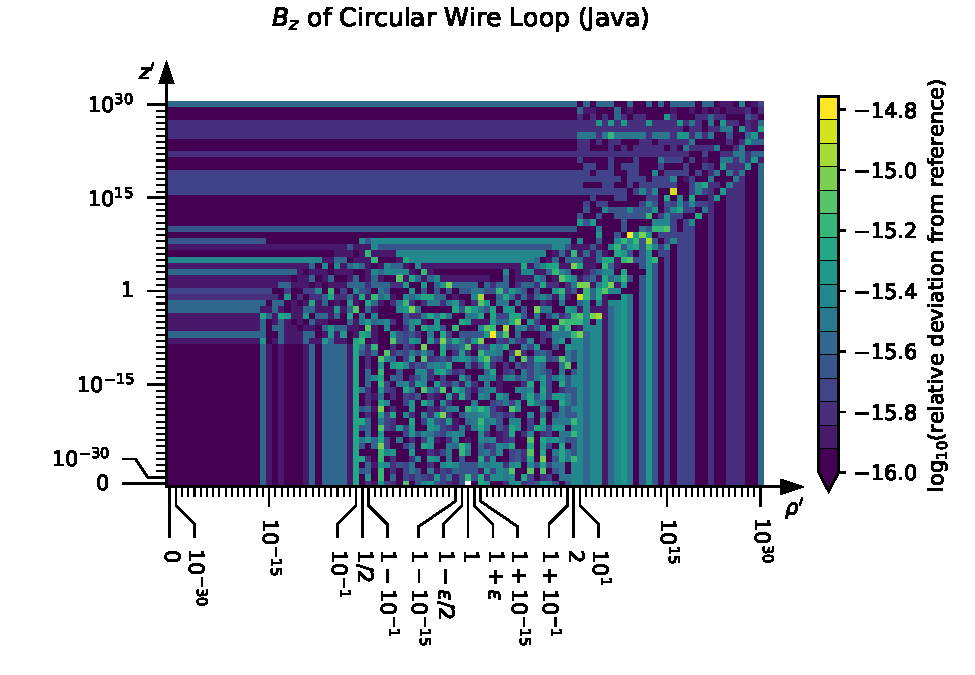
\includegraphics[width=0.8\textwidth]{img/CircularWireLoop_B_z_Java.pdf}
 \caption{Deviation between Java implementation of \eqn{cwl_B_z_switchover} and \eqn{B_z_ref}
          for the computation of $\tilde{B}_z$ of a circular wire loop
          in the error metric given by~\eqn{error_metric}.}
 \label{fig:CircularWireLoop_B_z_Java}
\end{figure}

\subsection{Further tests}

A second-order correction to the polygon approximation
for a circular wire loop~\cite{mcgreivy_2021} was tested.
\begin{figure}[htbp]
 \centering
 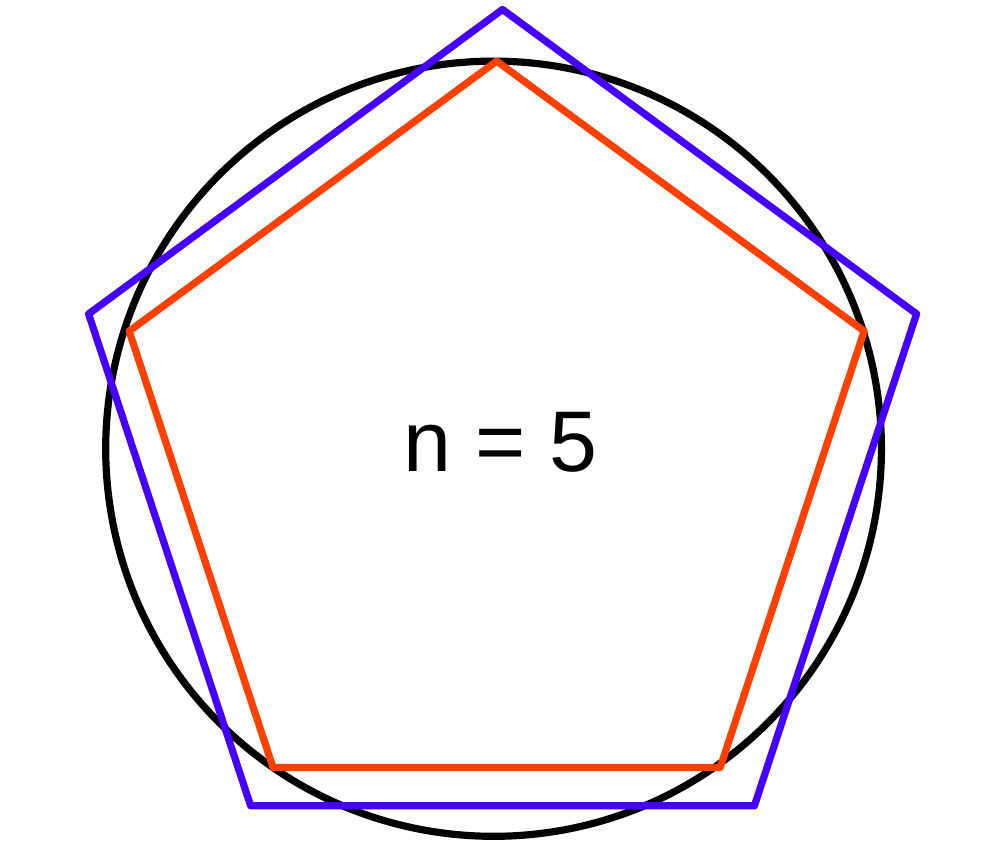
\includegraphics[width=0.5\textwidth]{img/sketch_McGreivy.png}
 \caption{Sketch of the McGreivy test setup.}
 \label{fig:sketch_McGreivy}
\end{figure}
Second-order iterative Kahan-Babuska summation~\cite{klein_2006} had to be used
to achive convergence down to numerical accuracy.
\begin{figure}[htbp]
 \centering
 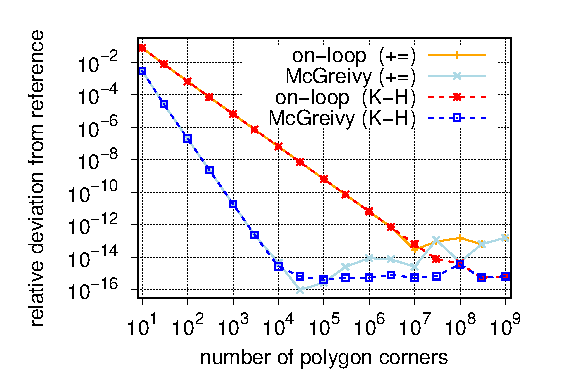
\includegraphics[width=0.8\textwidth]{img/McGreivy_convergence_2.eps}
 \caption{Convergence of the McGreivy test setup.}
 \label{fig:McGreivy_convergence_2}
\end{figure}
